\documentclass{beamer}
\usetheme{Madrid}
\usepackage{physics}
\usepackage{amsmath}
\usepackage{ragged2e}
\graphicspath{ {./images/} }

\newcommand\myheading[1]{%
  \par\bigskip
  {\Large\bfseries#1}\par\smallskip}

\title{Introduction to Logistic Regression and PCA}
\author{by Talentsprint Pvt. Ltd.}
\centering
\date{September 2020}

\begin{document}
\maketitle
\begin{frame}{Content}
	\begin{itemize}
		\item Logistic Regression
		\item Why not use Linear Regression?
		\item Fundamental Terms of Logistic Regression
		\item Estimating Probabilities
		\item Cost Function
		\item Pros and Cons
		\item Curse of Dimensionality
		\item Principal Component Analysis
		\item Example of PCA
	\end{itemize}
\end{frame}

\begin{frame}{Logistic Regression}
\begin{flushleft}
\begin{itemize}
	\item Logistic Regression (also called Logit Regression) is commonly used to estimate the probability that an instance belongs to a particular class (e.g., what is the probability that this email is spam?).
	\item If the estimated probability is greater than 50\%, then the model predicts that the instance belongs to that class (called the positive class, labeled “1”), or else it predicts that it does not (i.e., it belongs to the negative class, labeled “0”). This makes it a binary classifier.
\end{itemize}
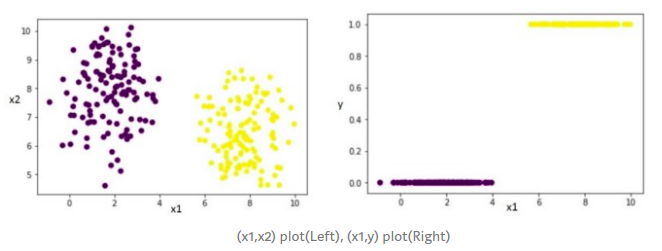
\includegraphics[scale=0.5]{Logistic_reg}\\
\end{flushleft}
\end{frame}

\begin{frame}{Why not use Linear Regression?}
	\begin{flushleft}
		Suppose we have a data of tumor size vs its malignancy. As it is a classification problem, if we plot, we can see, all the values will lie on 0 and 1. And if we fit best found regression line, by assuming the threshold at 0.5, we can do line pretty reasonable job.
		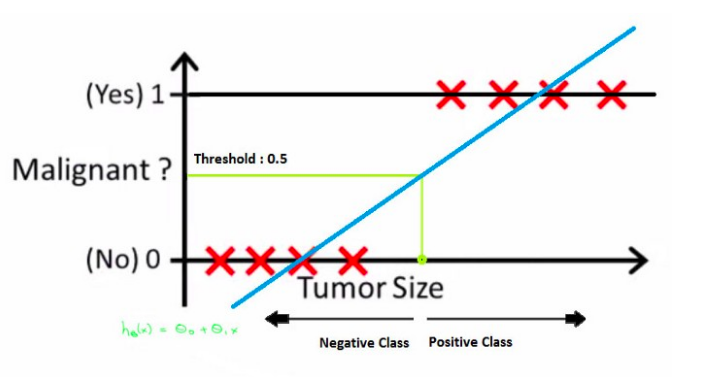
\includegraphics[scale=0.3]{Log_reg_2}\\
		We can decide the point on the x axis from where all the values lie to its left side are considered as negative class and all the values lie to its right side are positive class.
	\end{flushleft}
\end{frame}

\begin{frame}{Contd...}
\begin{flushleft}
But what if there is an outlier in the data. Things would get pretty messy. For example, for 0.5 threshold,\\
	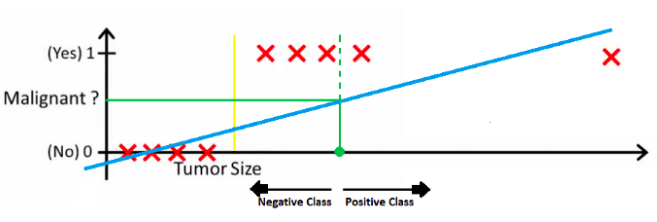
\includegraphics[scale=0.48]{Log_reg_3}\\
	If we fit best found regression line, it still won’t be enough to decide any point by which we can differentiate classes. It will put some positive class examples into negative class. The green dotted line (Decision Boundary) is dividing malignant tumors from benign tumors but the line should have been at a yellow line which is clearly dividing the positive and negative examples. So just a single outlier is disturbing the whole linear regression.
\end{flushleft}
\end{frame}

\begin{frame}{Fundamental Terms of Logistic Regression}
\begin{flushleft}
\myheading{Probability:}
		The probability that an event will occur is the fraction of times you expect to see that event in many trials. If the probability of an event occurring is Y, then the probability of the event not occurring is 1-Y. Probabilities always range between 0 and 1.
\myheading{Odds:}
	The odds are defined as the probability that the event will occur divided by the probability that the event will not occur. Unlike probability, the odds are not constrained to lie between 0 and 1 but can take any value from zero to infinity.\\
\vspace{10pt}
If the probability of Success is P, then the odds of that event is:
\begin{equation*}
	odds = \frac{P}{1-P}
\end{equation*}
\end{flushleft}
\end{frame}

\begin{frame}{Contd...}
\begin{flushleft}
	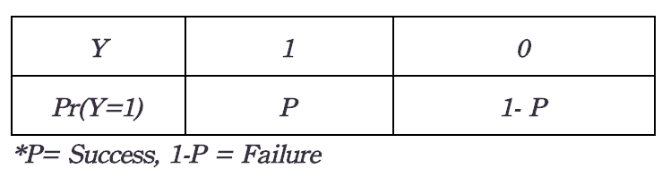
\includegraphics[scale=0.5]{table}
		\textbf{Example:} If the probability of success (P) is 0.60 (60\%), then the probability of failure(1-P) is 1–0.60 = 0.40(40\%). Then the odds are 0.60 / (1–0.60) = 0.60/0.40 = 1.5.

\end{flushleft}
\end{frame}

\begin{frame}{Estimating Probabilities}
\begin{flushleft}
Just like a Linear Regression model, a Logistic Regression
model computes a weighted sum of the input features (plus a bias term), but instead of outputting the result directly like the Linear Regression model does, it outputs the logistic of this result.
\begin{equation*}
	\hat{p} = h_\theta(x) = \sigma(\theta^Tx)
\end{equation*}
The logistic—noted σ(·)—is a sigmoid function (i.e., S-shaped) that outputs a number between 0 and 1.
\begin{equation*}
	\sigma(t) = \frac{1}{1 + e^{(-t)}}
\end{equation*}
Let’s consider t as linear function in a univariate regression model.
\begin{equation*}
	t = \theta^Tx = \theta_0 + \theta_1x_1 + \theta_2x_2 ....\theta_nx_n
\end{equation*}
Thus, 
\begin{equation*}
	\sigma(t) = \frac{1}{1 + e^{(-\theta^Tx)}} = \frac{1}{1 + e^{(\theta_0 + \theta_1x_1 + \theta_2x_2 ....\theta_nx_n)}}
\end{equation*}
	\end{flushleft}
\end{frame}
\begin{frame}{Contd...}
\begin{flushleft}
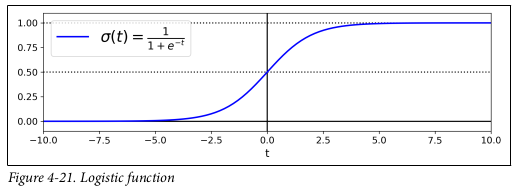
\includegraphics[scale=0.62]{sigmoid}\\
	 Once the Logistic Regression model has estimated the probability p = h θ (x) that an instance x belongs to the positive class, it can make its prediction ŷ easily,
\begin{equation*}
	\hat{p} = 
	\begin{cases}
		0,& \text{if } \hat{p} < 0.5 \\
		1,& \text{if } \hat{p} \geq 0.5
	\end{cases}
\end{equation*}
Notice that σ(t) < 0.5 when t < 0, and σ(t) ≥ 0.5 when t ≥ 0, so a Logistic Regression model predicts 1 if $\theta^Tx$ is positive, and 0 if it is negative.
\end{flushleft}
\end{frame}

\begin{frame}{Cost Function}
\begin{flushleft}
The objective of training is to set the param‐
eter vector θ so that the model estimates high probabilities for positive instances (y =1) and low probabilities for negative instances (y = 0). This idea is captured by the cost function for a single training instance,
\begin{equation*}
	c(\theta) = 
	\begin{cases}
		-\log(\hat{p}),& \text{if } y = 1\\
		-\log(1-\hat{p}),& \text{if } y = 0
	\end{cases}
\end{equation*}
\begin{itemize}
	\item This cost function makes sense because $-\log(t)$ grows very large when t approaches 0, so the cost will be large if the model estimates a probability close to 0 for a positive instance, and it will also be very large if the model estimates a probability close to 1 for a negative instance. 
	\item On the other hand, $-\log(t)$ is close to 0 when t is close to 1, so
the cost will be close to 0 if the estimated probability is close to 0 for a negative instance or close to 1 for a positive instance.
\end{itemize}
	\end{flushleft}
\end{frame}

\begin{frame}{Contd...}
\begin{flushleft}
The cost function over the whole training set is simply the average cost over all training instances. It can be written in a single expression (as you can verify easily), called the log loss,
\begin{equation*}
	J(\theta) = -\frac{1}{m}\sum_{i=1}^{m}\bigg[y^{(i)}\log\Big(p^{(i)}\Big)+\Big(1-y^{(i)}\Big)\log\Big(1 - p^{(i)}\Big)\bigg]
\end{equation*}

The partial derivatives of the cost function with regards to the $j^th$ model parameter $\theta_j$ is given by
\begin{equation*}
	\pdv{}{\theta_j}J(\theta) = \frac{1}{m}\sum_{i=1}^{m}\Big(\sigma\Big(\theta^Tx^{(i)}\Big)-y^{(i)}\Big)x_j^{(i)}
\end{equation*}
For each instance it computes the prediction error and multiplies it by the $j^th$ feature value, and then it computes the average over all training instances. Once the gradient vector containing all the partial derivatives is found it can be used in the Batch Gradient Descent algorithm or Stochastic GD or Mini-batch GD according to the need.
\end{flushleft}
\end{frame}

\begin{frame}{Pros and Cons}
\begin{flushleft}
\myheading{Pros:}
\begin{itemize}
	\item Simple and easy implementations.
	\item For small datasets, less prone to Overfitting.
	\item Very efficient when dataset has features that are linearly separable.
	\item Can easily be extended to Multiclass classification using Softmax classifier.
	\item Training time is very quick.
\end{itemize}
\myheading{Cons:}
\begin{itemize}
	\item On high dimensional datasets, model over-fits on the training set.
	\item Non linear problems can't be solved.
	\item Large dataset is required for efficient model training.
	\item Requires moderate or no multicollinearity between independent variables.
	\item Difficult to capture complex relationships.
\end{itemize}
\end{flushleft}
\end{frame}

\begin{frame}{Curse of Dimensionality}
	\begin{flushleft}
		The curse of dimensionality refers to the phenomena that occur when classifying, organizing, and analyzing high dimensional data that does not occur in low dimensional spaces, specifically the issue of data sparsity and “closeness” of data.\\
		Sparsity of data occurs when moving to higher dimensions. the volume of the space represented grows so quickly that the data cannot keep up and thus becomes sparse, as seen below.\\

	\end{flushleft}
	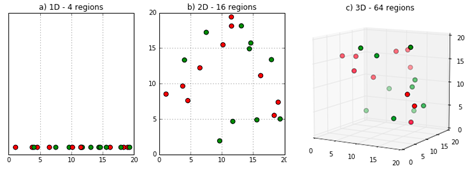
\includegraphics[scale=0.4]{cod}\\
\begin{flushleft}
	As the data space seen above moves from one dimension to two dimensions and finally to three dimensions, the given data fills less and less of the data space and the data for analysis grows exponentially.
\end{flushleft}
\end{frame}

\begin{frame}{Principal Component Analysis}
	\begin{flushleft}
	\myheading{Introduction}
	The central idea of principal component analysis (PCA) is to reduce the dimensionality of a data set consisting of a large number of interrelated variables while retaining as much as possible of the variation present in the data set. This is achieved by transforming to a new set of variables, the principal components (PCs), which are uncorrelated, and which are ordered so that the first few retain most of the variation present in all of the original variables.\\
\vspace{10pt}
\myheading{Math behind PCA}
PCA can be thought of as an unsupervised learning problem. The whole process of obtaining principle components from a raw dataset can be simplified in six parts :
	\end{flushleft}
\end{frame}

\begin{frame}{Contd...}
	\begin{flushleft}
	\begin{itemize}
		\item Take the whole dataset consisting of d+1 dimensions and ignore the labels such that our new dataset becomes d dimensional.
		\item Compute the mean for every dimension of the whole dataset.
		\item Compute the covariance matrix of the whole dataset.
		\item Compute eigenvectors and the corresponding eigenvalues.
		\item Sort the eigenvectors by decreasing eigenvalues and choose k eigenvectors with the largest eigenvalues to form a d x k dimensional matrix W.
		\item Use this d x k eigenvector matrix to transform the samples onto the new subspace.
	\end{itemize}
\end{flushleft}
\end{frame}

\begin{frame}{Example of PCA}
	\begin{flushleft}
Let our data matrix X be the score of five students :
	\begin{itemize}
	\item Take the whole dataset consisting of d+1 dimensions and ignore the labels such that our new dataset becomes d dimensional.
	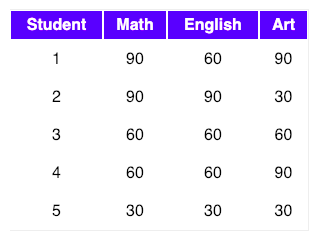
\includegraphics[scale=0.4]{data}\\
	\item Compute the mean of every dimension of the whole dataset.
	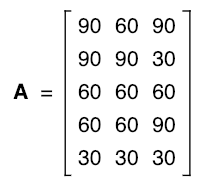
\includegraphics[scale=0.4]{matrixA}\\
	\end{itemize}
\end{flushleft}
\end{frame}

\begin{frame}{Contd...}
	\begin{flushleft}
	Mean of Matrix A would be,\\
	\end{flushleft}
	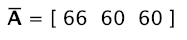
\includegraphics[scale=0.4]{meanA}\\
	\begin{itemize}
	\item Compute the covariance matrix of the whole dataset ( sometimes also called as the variance-covariance matrix).
	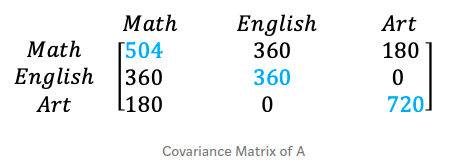
\includegraphics[scale=0.4]{covarianceA}\\
	\item Compute Eigenvectors and corresponding Eigenvalues
	\end{itemize}
	\begin{equation*}
		-\lambda^3 + 1584\lambda^2 - 641520\lambda + 25660800 = 0
	\end{equation*}
	\begin{equation*}
		\lambda_1 = 44.81966, \lambda_2 = 629.11039, \lambda_3 = 910.06995
	\end{equation*}
	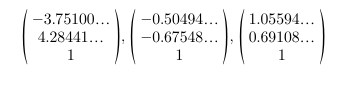
\includegraphics[scale=0.5]{eigen_vec}
\end{frame}

\begin{frame}{Contd...}
	\begin{itemize}
	\item Sort the eigenvectors by decreasing eigenvalues and choose k eigenvectors with the largest eigenvalues to form a d x k dimensional matrix W.\\
	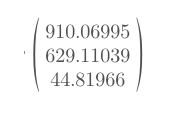
\includegraphics[scale=0.5]{eigen_vec1}\\
	So Eigen vectors corresponding to two maximum eigenvalues are,
	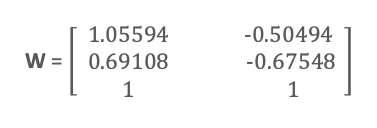
\includegraphics[scale=0.4]{eigen_vec2}\\
	\item Transform the samples onto the new subspace.
	In the last step, we use the 3 x 2 dimensional matrix W that we just computed to transform our samples onto the new subspace via the equation y = $W' . x$ where W′ is the transpose of the matrix W.
	\end{itemize}
\end{frame}
\begin{frame}
\huge{\centerline{The End}}
\end{frame}
\end{document}